\cleardoublepage
\chapter{KEBIJAKAN PRIVASI DAN MANAJEMEN DARURAT (WAWANCARA 5)}
\label{chap:lampiran_e}

\section{Dokumentasi Foto Wawancara 5}
Berikut adalah dokumentasi visual pada saat diskusi mengenai kebijakan privasi, notifikasi, dan prosedur darurat evakuasi.

\begin{figure}[htbp]
    \centering
    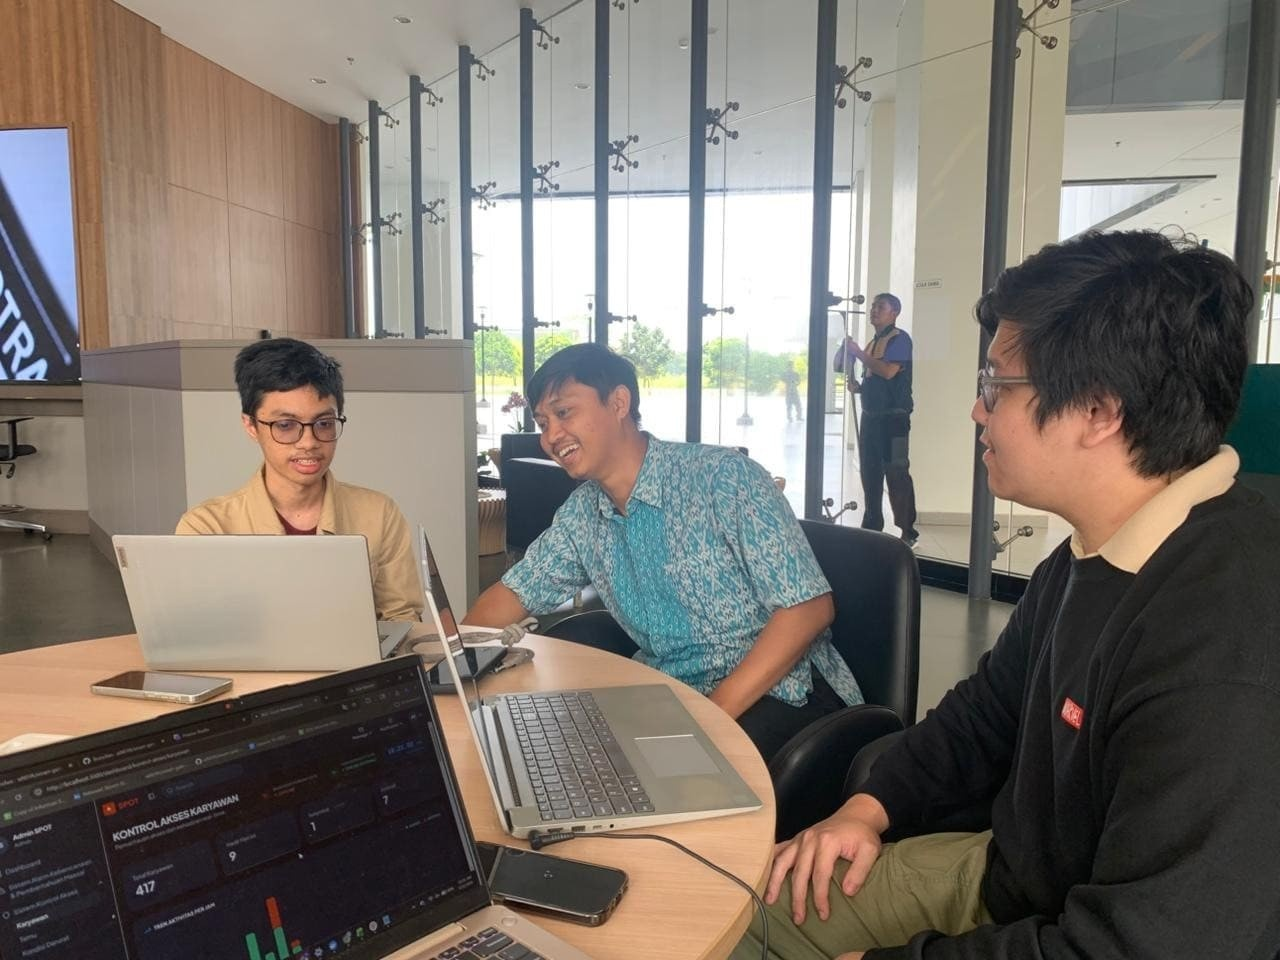
\includegraphics[width=0.6\textwidth]{images/wawancara5_1.png}
    \caption{Dokumentasi Pelaksanaan Wawancara 5 (E)}
\end{figure}

\section{Transkrip Wawancara 5}
Wawancara kelima dilakukan untuk membahas aspek kebijakan perlindungan data, fitur kendali operasional jarak jauh, serta kebutuhan sistem saat kondisi darurat/evakuasi. Berikut adalah transkrip lengkap dari diskusi tersebut:

\begin{longtable}{|c|p{0.35\textwidth}|p{0.55\textwidth}|}
\hline
\textbf{No} & \textbf{Pewawancara (Mahasiswa)} & \textbf{Narasumber (Kepala Seksi Data \& SI DKST)} \\ \hline
\endfirsthead
\hline
\textbf{No} & \textbf{Pewawancara (Mahasiswa)} & \textbf{Narasumber (Kepala Seksi Data \& SI DKST)} \\ \hline
\endhead
\hline
\endfoot
\hline
\endlastfoot
1 & Untuk tampilan data di \textit{dashboard}, apakah perlu disensor atau di-\textit{pseudonymize} namanya untuk menjaga privasi? & Tidak perlu, pakai nama asli saja (sesuai yang terdaftar di mesin) tidak masalah. \textit{Dashboard} ini kan privasinya untuk pihak internal manajemen/satpam, jadi mereka harus tahu nama aslinya. Yang tidak perlu ditampilkan mungkin ID unik mesinnya saja, karena itu tidak ada urgensinya untuk dibaca. \\ \hline
2 & Berarti informasi apa yang paling penting untuk dimunculkan pada daftar pergerakan tersebut? & Nama orangnya, dia masuk dari pintu/lobi sebelah mana, jam masuk, dan jam keluar. Kalau bisa nanti ditambah fitur untuk mendeteksi apakah orang ini karyawan dari tenant yang mana, itu akan sangat membantu pendataan. \\ \hline
3 & Kami berencana membuat fitur kendali buka-tutup gerbang secara \textit{remote} (jarak jauh) dari \textit{dashboard}, apakah ini berguna? & Itu sangat bagus. Jadi satpam atau resepsionis bisa membukakan akses gerbang langsung dari klik di komputer \textit{dashboard}, tanpa harus mendatangi alatnya secara fisik. Ini sangat membantu misalnya untuk skenario kedatangan tamu prioritas. \\ \hline
4 & Untuk notifikasi kejadian anomali (akses gagal/tidak dikenal), apakah sebaiknya sistem menangkap dan menampilkan fotonya? & Iya, harusnya begitu. Ketika ada yang gagal (\textit{access denied}), fotonya diambil dan ditampilkan supaya satpam tahu siapa yang mencoba masuk sembarangan. \\ \hline
5 & Kalau untuk log akses yang sukses/normal, apakah fotonya juga perlu ditampilkan di \textit{dashboard}? & Tidak usah. Kalau dia masuk secara normal dan namanya sudah sesuai, biarkan saja log waktunya tercatat di database tanpa perlu menampilkan rekaman mukanya di layar utama \textit{dashboard}. Itu untuk menjaga privasi. Jadi yang fotonya ditampilkan cukup untuk kejadian yang salah/eror (anomali) saja. \\ \hline
6 & Untuk fitur notifikasi, Bapak sempat menyebut soal WhatsApp. Apakah kami harus pakai itu? & WhatsApp bagus, tapi harus langganan API berbayar. Saran saya, coba integrasikan dengan Telegram Bot saja karena gratis. Nanti notifikasi \textit{error}, gerbang \textit{offline}, atau peringatan anomali bisa langsung ditembak ke grup Telegram yang isinya satpam-satpam gedung. \\ \hline
7 & Kalau saat kondisi darurat/evakuasi, tampilan \textit{dashboard}-nya harusnya seperti apa, Pak? & Menu untuk kondisi darurat sebaiknya dipisah dari pemantauan normal. Saat darurat, \textit{dashboard} harusnya fokus menampilkan data "Siapa yang belum keluar dari gedung". Nanti petugas bisa mencocokkan jumlah orang yang terdata masih di dalam (\textit{dashboard}) dengan jumlah orang yang sudah sampai di titik kumpul (\textit{muster point}). \\ \hline
\end{longtable}
